\begin{enumerate}[label=\thesubsection.\arabic*.,ref=\thesubsection.\theenumi]
\numberwithin{equation}{enumi}

\item Consider a state-variable model of a system 
\begin{align}
\myvec{\dot{x_{1}}\\\dot{x_{2}}}
=
\myvec{0&1\\-\alpha&-2\beta}\myvec{x_{1}\\x_{2}}
+
\myvec{b_{1}\\b_{2}}  r
\end{align}
\begin{align}
y
=
\myvec{1&0}\myvec{x_{1}\\x_{2}}
\end{align}
where y is the output, and r is the input.
%
Find the the system transfer function $H(s)$.

\solution The state space model is given by
\begin{align}
\dot{X} = AX + BU
\end{align}
\begin{align}
Y = CX + DU
\end{align}
%
From \eqref{eq:x_init} we know that the transfer function for the state space model is:
\begin{align}
H(s) = C(sI - A)^{-1}B + D
\end{align}
\begin{align}
\implies H(s) = \frac
{
\myvec{1&0}\myvec{s+2\beta&1\\-\alpha&s}\myvec{b_{1}\\b_{2}}
}
{
s(s+2\beta) + \alpha
}
\end{align}
\begin{align}
= \LARGE{\frac{b_{1}(s+2\beta) + b_{2}}{s^{2}+2s\beta+\alpha}}
\end{align}
\begin{align}
   \implies H(s) = \LARGE{\frac{b_{1}s}{s^{2}+2s\beta+\alpha}} + \LARGE{\frac{2b_{1}\beta + b_{2}}{s^{2}+2s\beta+\alpha}}
\end{align}
%\begin{table}[!ht]
%\centering
%\begin{enumerate}[label=\thesection.\arabic*.,ref=\thesection.\theenumi]
\numberwithin{equation}{enumi}

\item Consider a state-variable model of a system 
\begin{align}
\myvec{\dot{x_{1}}\\\dot{x_{2}}}
=
\myvec{0&1\\-\alpha&-2\beta}\myvec{x_{1}\\x_{2}}
+
\myvec{b_{1}\\b_{2}}  r
\end{align}
\begin{align}
y
=
\myvec{1&0}\myvec{x_{1}\\x_{2}}
\end{align}
where y is the output, and r is the input.
%
Find the Damping ratio $\zeta$ and the Undamped natural frequency $\omega_{n}$ of the system.

\solution The state space model is given by
\begin{align}
\dot{X} = AX + BU
\end{align}
\begin{align}
Y = CX + DU
\end{align}
%
The transfer function for the state space model is:
\begin{align}
H(s) = C(sI - A)^{-1}B + D
\end{align}
\begin{align}
\implies H(s) = \frac{\myvec{1&0}\myvec{s+2\beta&1\\-\alpha&s}\myvec{{b_{1}\\b_{2}}}}{s(s+2\beta) + \alpha}
\end{align}
\begin{align}
= \LARGE{\frac{b_{1}(s+2\beta) + b_{2}}{s^{2}+2s\beta+\alpha}}
\end{align}
\begin{align}
   \implies H(s) = \LARGE{\frac{b_{1}s}{s^{2}+2s\beta+\alpha}} + \LARGE{\frac{2b_{1}\beta + b_{2}}{s^{2}+2s\beta+\alpha}}
\end{align}
Generally for a second order system the transfer function is given by
\begin{align}
H(s) = \LARGE{\frac{\omega_{n}^2}{s^{2}+2s\zeta\omega_{n}+\omega_{n}^2}}
\end{align}
Now from the transfer function we got we can see that our system is bandpass and lowpass combination but the comaprison of denominator of our transfer function to the general transfer function is still valid.
\begin{align}
\therefore 2\zeta\omega_{n} = 2\beta,
\end{align}
\begin{align}
\omega_{n}^2 = \alpha
\end{align}
\begin{align}
\implies \zeta = \frac{\beta}{\sqrt{\alpha}} , \omega_{n} = \sqrt{\alpha}
\end{align}
\end{enumerate}


%\caption{}
%\label{table:ee18btech11011}
%\end{table}
\item Find the Damping ratio $\zeta$ and the Undamped natural frequency $\omega_{n}$ of the system.
\\
\solution
Generally for a second order system the transfer function is given by
\begin{align}
H(s) = \LARGE{\frac{\omega_{n}^2}{s^{2}+2s\zeta\omega_{n}+\omega_{n}^2}}
\end{align}
Now from the transfer function we got we can see that our system is bandpass and lowpass combination but the comaprison of denominator of our transfer function to the general transfer function is still valid.
\begin{align}
\therefore 2\zeta\omega_{n} = 2\beta,
\end{align}
\begin{align}
\omega_{n}^2 = \alpha
\end{align}
\begin{align}
\implies \zeta = \frac{\beta}{\sqrt{\alpha}} , \omega_{n} = \sqrt{\alpha}
\end{align}
\item What is the significance of $\zeta$ and  $\omega_{n}$? Explain through plots.
\solution 
\begin{center}
\begin{tabular}{ | m{3.5cm} | m{3.5cm}| } 
\hline
Damping Ratio & Undamped Natural Frequency \\ 
\hline
Damping ratio basically indicates the amount of damping present in the overall system. & It's the frequency of oscillation of the system without damping. \\ 
\hline
\item $\zeta$ \textgreater 1 $\implies$ Overdamped system
\item $\zeta$ = 1 $\implies$ Critically damped system
\item 0 \textless $\zeta$ \textless 1 $\implies$ Underdamped system
\item $\zeta$ = 0 $\implies$ Undamped system & Only systems with $\zeta$ \textless 1 have a natural frequency $\omega$ and only in the case that $\zeta$ = 0 will the natural frequency $\omega$ = $\omega_{n}$, the undamped natural frequency. \\ 
\hline
\end{tabular}
\end{center}
Given above is a table explaining about $\zeta$ , $\omega_n$ and below is a plot explaining what happens if zeta increases. If zeta increases than the magnitude decreases as shown in the Fig.  \ref{fig:EE18btech11011}.
\begin{figure}[!ht]
	\begin{center}
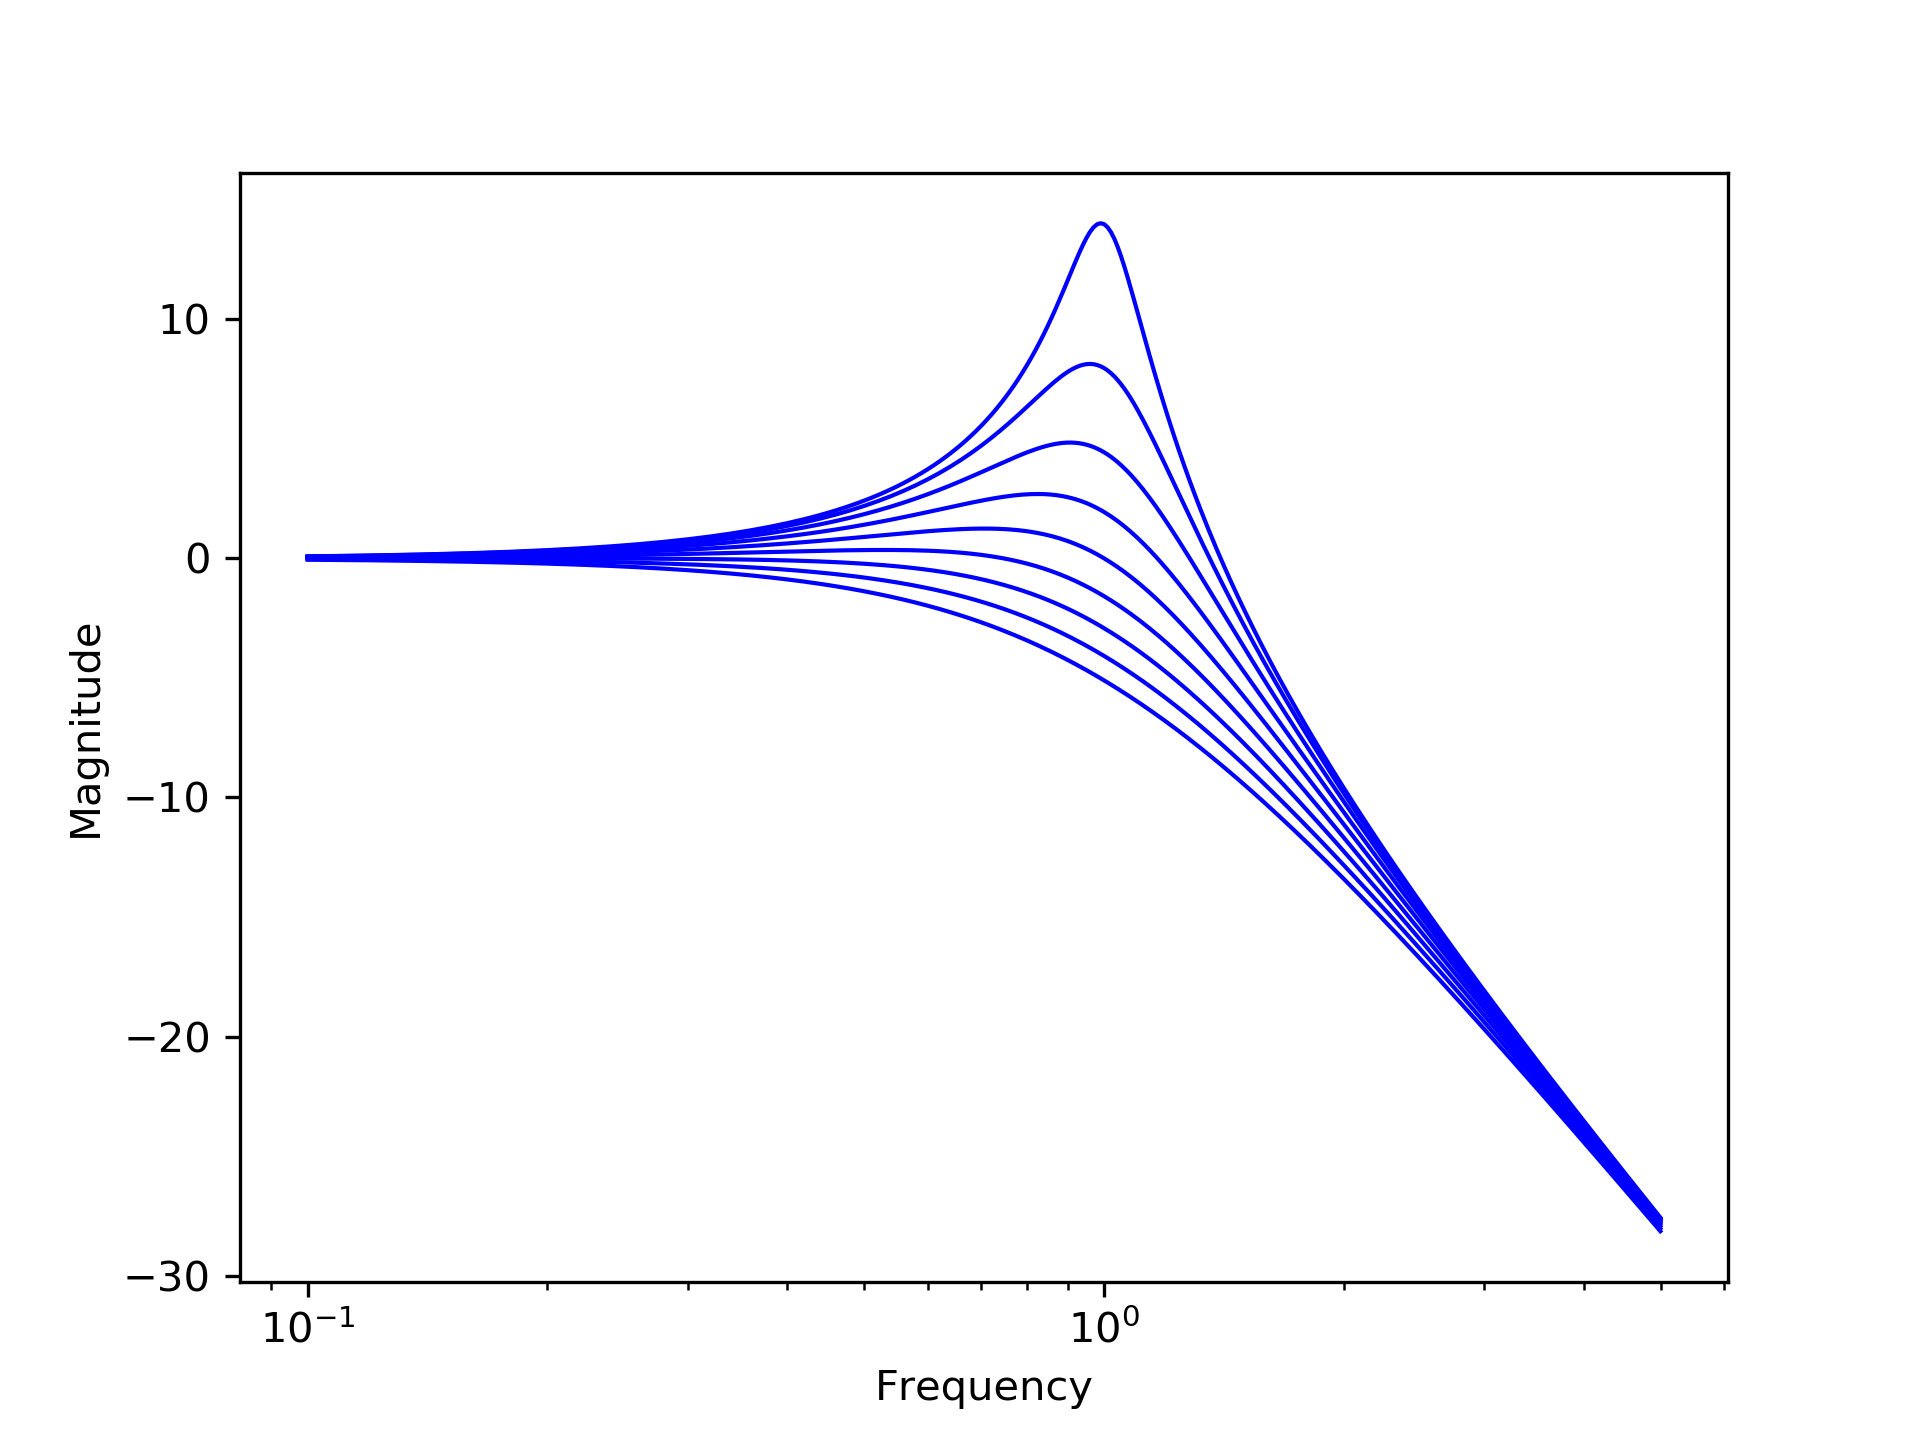
\includegraphics[width=\columnwidth]{EE18btech11011.png}		
	\end{center}
\caption{}
\label{fig:EE18btech11011}
\end{figure}
\item How do $\alpha$ and $\beta$ affect the system performance?  Explain through plots.
\\
\solution From the Fig.  \ref{fig:beta_constant} we can say that when $\beta$ is kept constant and $\alpha$ is increased than so as the magnitude decreases and from the Fig. \ref{fig:alpha_constant} we can say that when $\alpha$ is kept constant and $\beta$ is increased the magnitude is increased.
%
\begin{figure}[!ht]
	\begin{center}
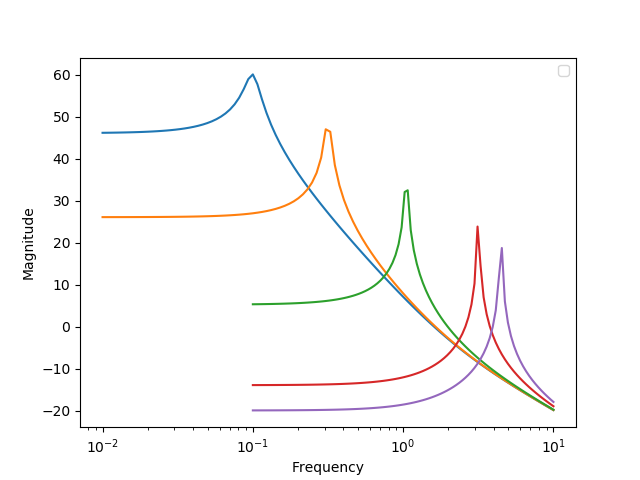
\includegraphics[width=\columnwidth]{beta_constant.png}		
	\end{center}
\caption{}
\label{fig:beta_constant}
\end{figure}
%
\begin{figure}[!ht]
	\begin{center}
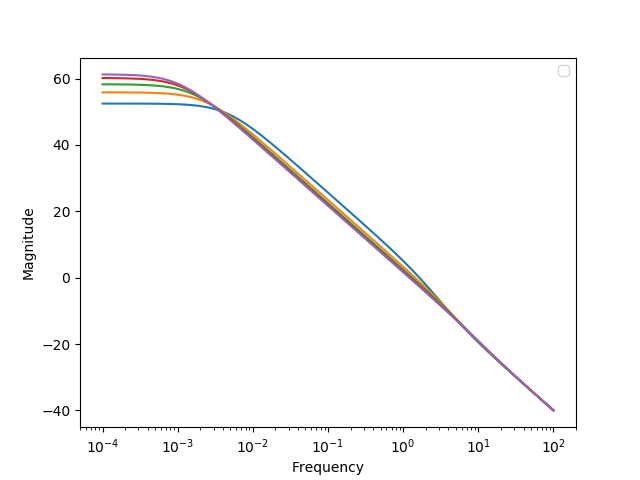
\includegraphics[width=\columnwidth]{alpha_constant.png}		
	\end{center}
\caption{}
\label{fig:alpha_constant}
\end{figure}

\end{enumerate}
